\section{Methodology Overview}
\label{sec:methodology-overview}

The research methodology is designed to address the research objectives mentioned in Section~\ref{subsec:research-questions-objectives}. This chapter first presents a general idea of the research process and then provides a detailed explanation of each stage, including how it was implemented and the experiments conducted at each step.

\begin{figure*}[h]
    \centering
    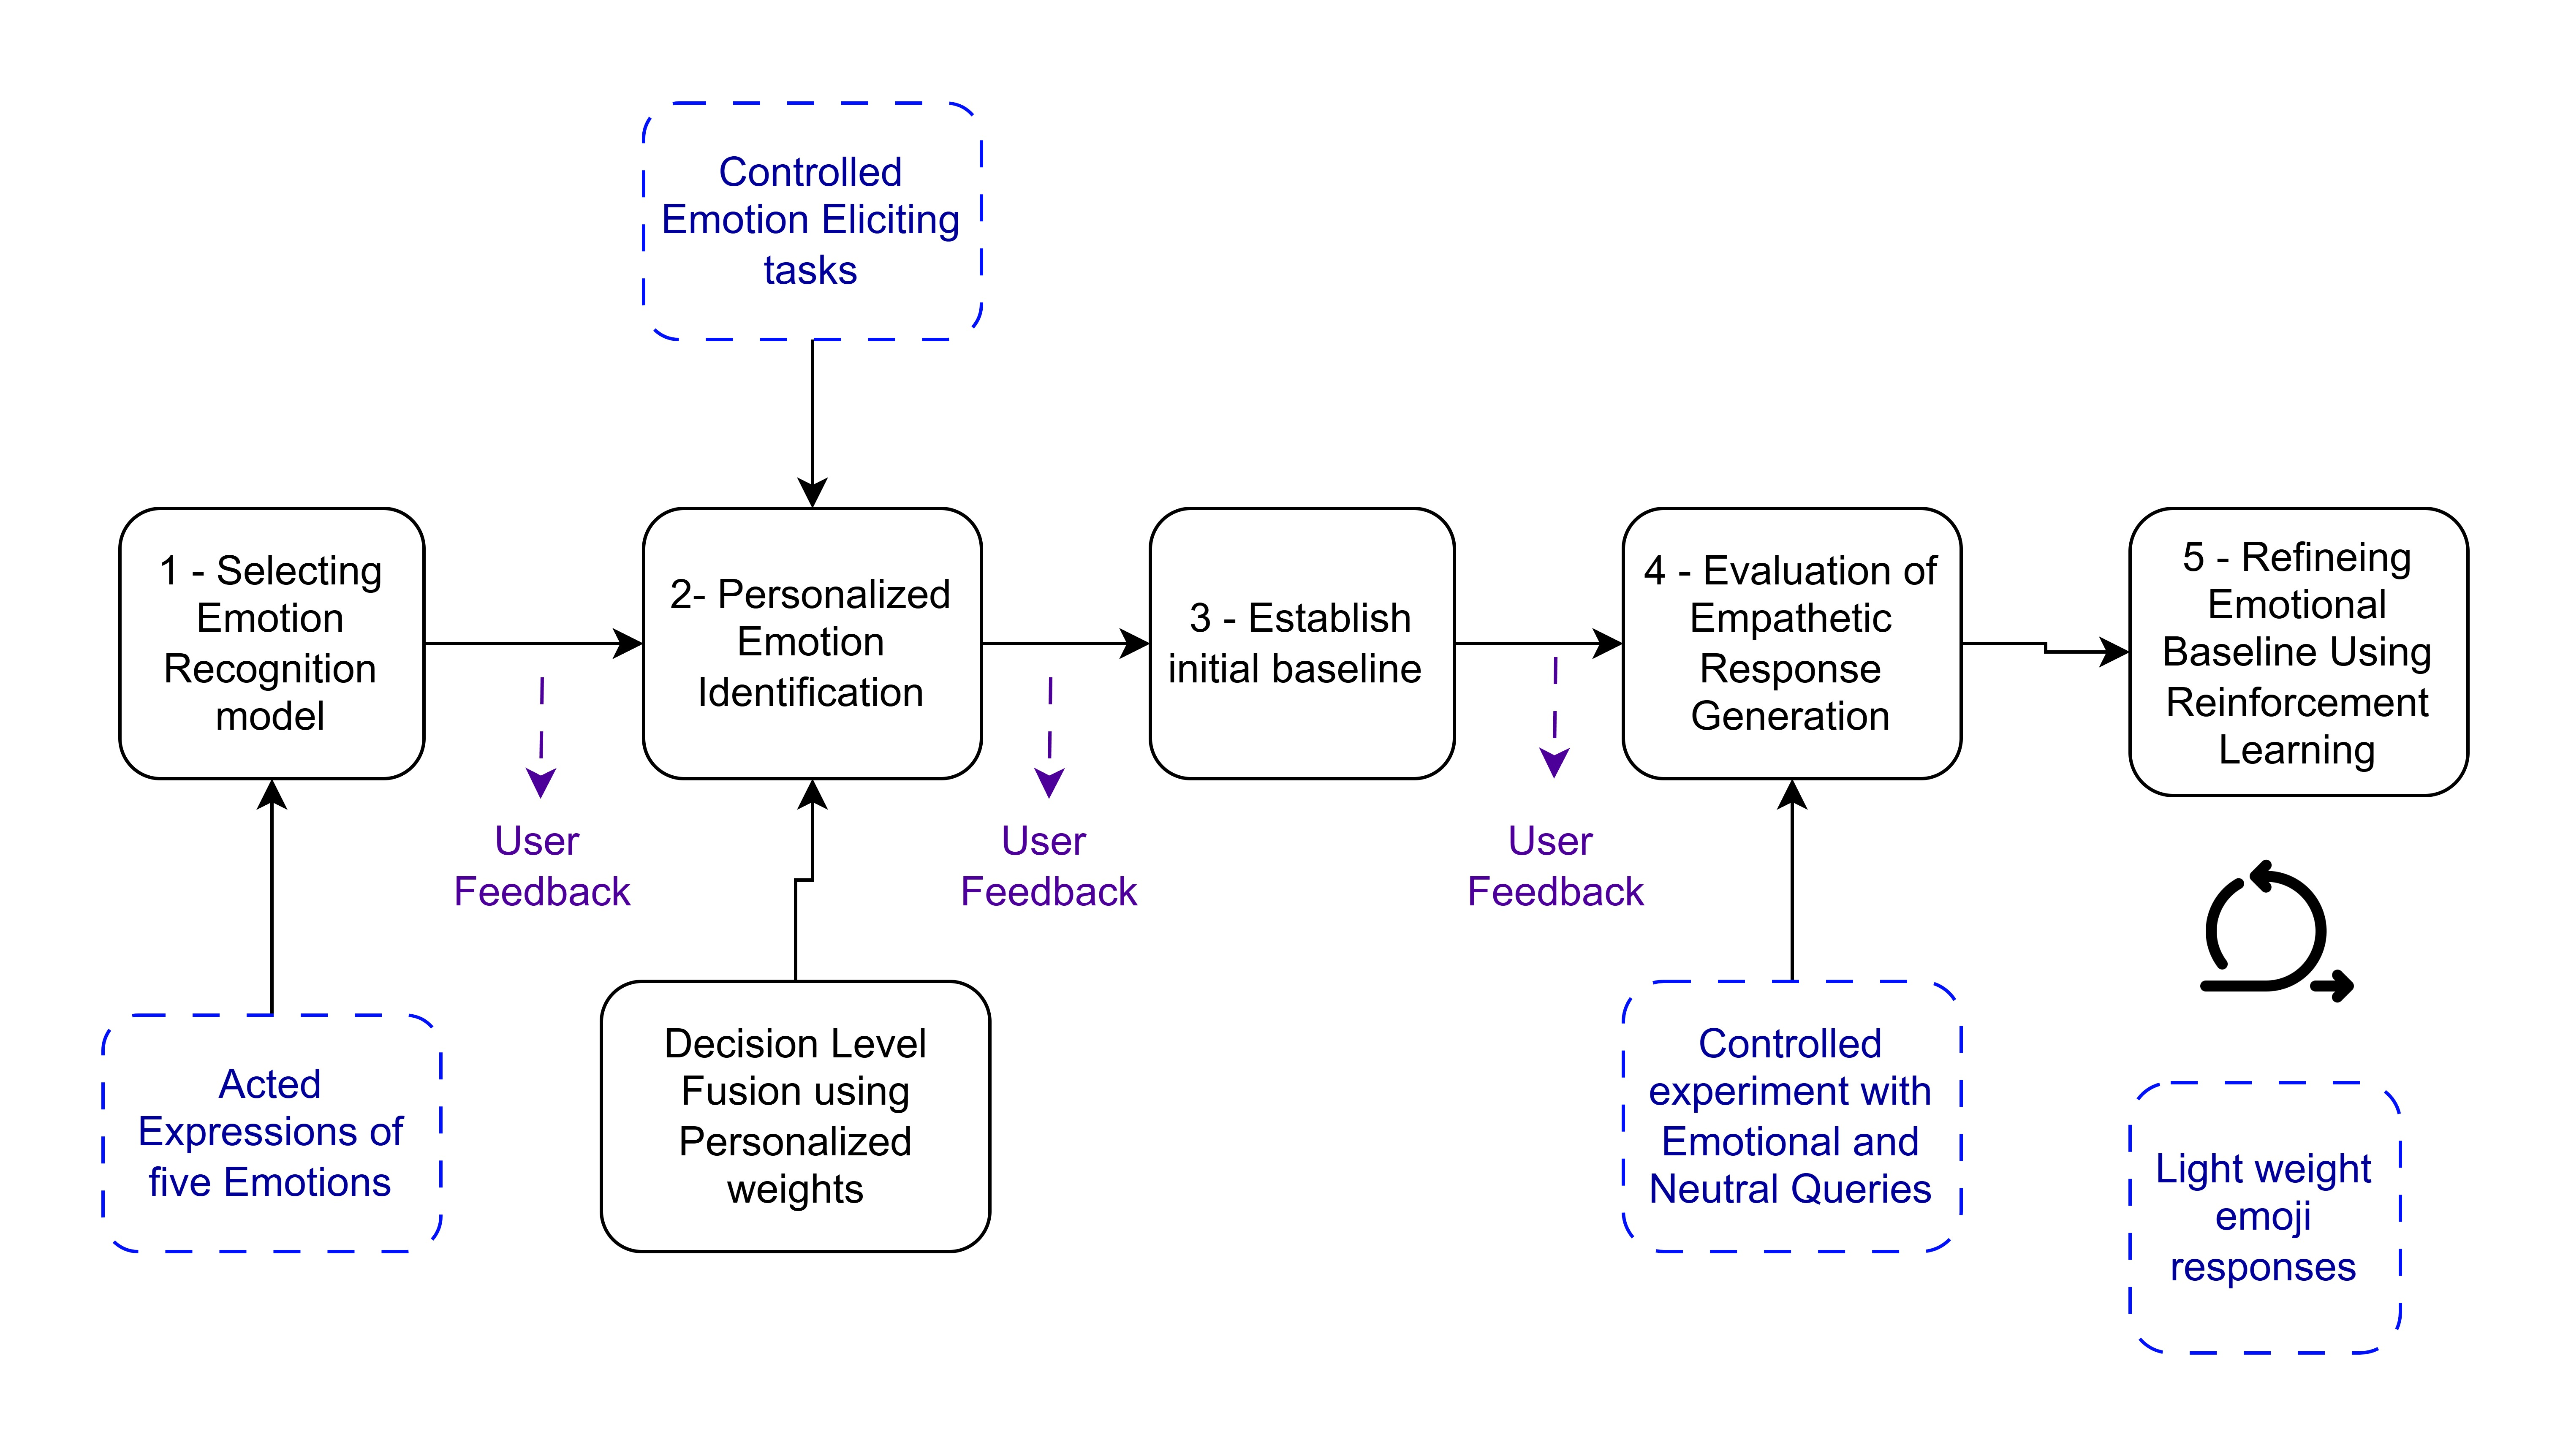
\includegraphics[width=1\textwidth]{img/chapter_03/methodology.jpg}
    \captionof{figure}{Main stages of the research methodology}
    \label{fig:design-stages}
\end{figure*}

The whole research is divided into five main stages. The overall design of these stages is illustrated in Figure~\ref{fig:design-stages}. Each stage is designed in a way that supports the next stage and contributes to the final objective of the research. A short overview of each stage is given below, and a more detailed explanation is provided in the following sections of this chapter.

\begin{enumerate}
    \item \textbf{Selecting emotion recognition model:} In this stage, the main focus is to identify effective models that can recognize human emotions using both facial expressions and speech signals. Several existing models were reviewed and tested to choose the most suitable ones to address \hyperref[rq:1.1]{Research Question 1.1}. 

    \item \textbf{Personalized emotion identification:} After selecting the models, the next step is to combine both facial and speech data for better emotion recognition. Also, the system is adjusted to consider individual differences by using dynamic weighting machanism by addressing \hyperref[rq:1.2]{Research Question 1.2}, making it more personalized.

    \item \textbf{Establish initial Baseline:} This stage involves setting up the Emotional Baseline which can be used to identify the emotional mood of the user to address \hyperref[rq:2.1]{Research Question 2.1}. The baseline is established using data collected from participants during emotion-eliciting tasks. The aim is to create a reference point for each participant that can be used to measure deviations in their emotional state.

    \item \textbf{Evaluation of Empathyic Response Generation:} In this stage, participants interact with a LLM by submitting their queries. Two types of responses are collected: one using the original query, and another combining the query with the user's current emotional state using prompt engineering. The goal of this stage is to observe how emotional context can influence the quality and personalization of responses given by the LLM. This stage is designed to address \hyperref[rq:3.1]{Research Question 3.1}.


    \item \textbf{Refining the Emotional Baseline using Reinforcement Learning:} Finally, the initial baseline is improved using reinforcement learning techniques by addressing \hyperref[rq:2.1]{Research Question 2.1}. This allows the system to learn and improve over time based on feedback and performance.

\end{enumerate}

Each of these stages will be discussed in detail in the following sections. Experiments, implementation methods, tools, and results related to each stage will also be described.

